\documentclass[12pt,a4paper]{article}
\usepackage[utf8]{inputenc}
\usepackage[portuguese]{babel}
\usepackage[T1]{fontenc}
\usepackage{amsmath}
\usepackage{amsfonts}
\usepackage{amssymb}
\usepackage{booktabs}
\usepackage{graphicx}
\usepackage[table,xcdraw]{xcolor}
%\usepackage{hyperref}
\usepackage[left=2cm,right=2cm,top=2cm,bottom=2cm]{geometry}
\author{Eduardo Adame}
\title{Primeiro Documento}
\begin{document}

\maketitle
\newpage

\tableofcontents
\newpage

\section{Primeiros Passos}
\subsection{Texto corrido}

Eu vou à praia todos os dias. % Texto corrido, basta escrever.

Eu estou mentindo. 40\% da população está acima do peso.
\subsection{Tipos e Tamanhos de Texto}
\subsubsection{Tipos de Texto}

Hoje foi um dia \textbf{MANEIRAÇO}, ouvi um \emph{senhor} falando aquela expressão em latim \textit{carpe diem}! 

Essa palavra está em \textbf{negrito}.

Eu adoro esse \textsc{tipo de letra}.
\subsubsection{Tamanhos de Texto}

Esse texto vai ficar {\Huge grande}

E esse aqui, {\tiny pequeno}.

\section{Listas}
\subsection{Listas Enumeradas}

\begin{enumerate}% NÃO PODE FICAR VAZIO
\item Carlos
\item Bruno
\item Fernando
\item[Last] Eduardo %DESCRIPTION
\end{enumerate}

\subsection{Listas Não Enumeradas}

\begin{itemize}
\item Carla
\item Bruna
\item Fernanda
\item Eduarda
\end{itemize}
\newpage


\subsection{Lista dentro de lista}
\label{ssc:ldl}
\begin{enumerate}
\item Nomes Masculinos
\begin{enumerate}
\item Eduardo
\item Marcelo
\item Fabiano
\end{enumerate}
\item Nomes Femininos
\begin{enumerate}
\item Eduarda
\item Marcela
\item Fabiana
\item Maria
\begin{enumerate}
\item Eduarda
\item Patrícia
\item Cláudia
\end{enumerate}
\end{enumerate}
\end{enumerate}


\section{Nota de Rodapé}

"Se você julgar um peixe pela sua capacidade de subir em uma árvore, ele vai passar a vida achando que é inútil."\footnote{EINSTEIN, Albert}

Eu estudo no CEFET/RJ\footnote{Centro Federal de Educação Tecnológica Celso Suckow da Fonseca}
	
\section{Matemática}

Para toda equação do segundo grau na forma $ax^2 + bx + c= 0$, suas raízes podem ser definidas por:

$$ x = \dfrac{-b \pm \overbrace{\sqrt{\Delta}}^{\sqrt{b^2 - 4 a c}}}{2a} $$
Sendo $\Delta = b^2 - 4 a c$

$$\sqrt[3]{8}=2$$

$$a^2 = b^2 + c^2 \,\ \therefore \,\ a = \sqrt{b^2 + c^2}$$

$$\text{Probabilidade} = \dfrac{\text{Casos Favoráveis}}{\text{Casos Totais}}$$

Condições de Equilíbrio:

$$\sum_{i=1}^{n} F_i = 0$$
$$\sum_{i=1}^{n} M_i = 0$$

Definição de Integral definida:

$$\int_a^b f(x)\, dx = F(b) - F(a)$$
$$\int x^n \, dx= \dfrac{x^{n+1}}{n+1} + C$$

\section{Figuras}
\subsection{Formatação Comum}

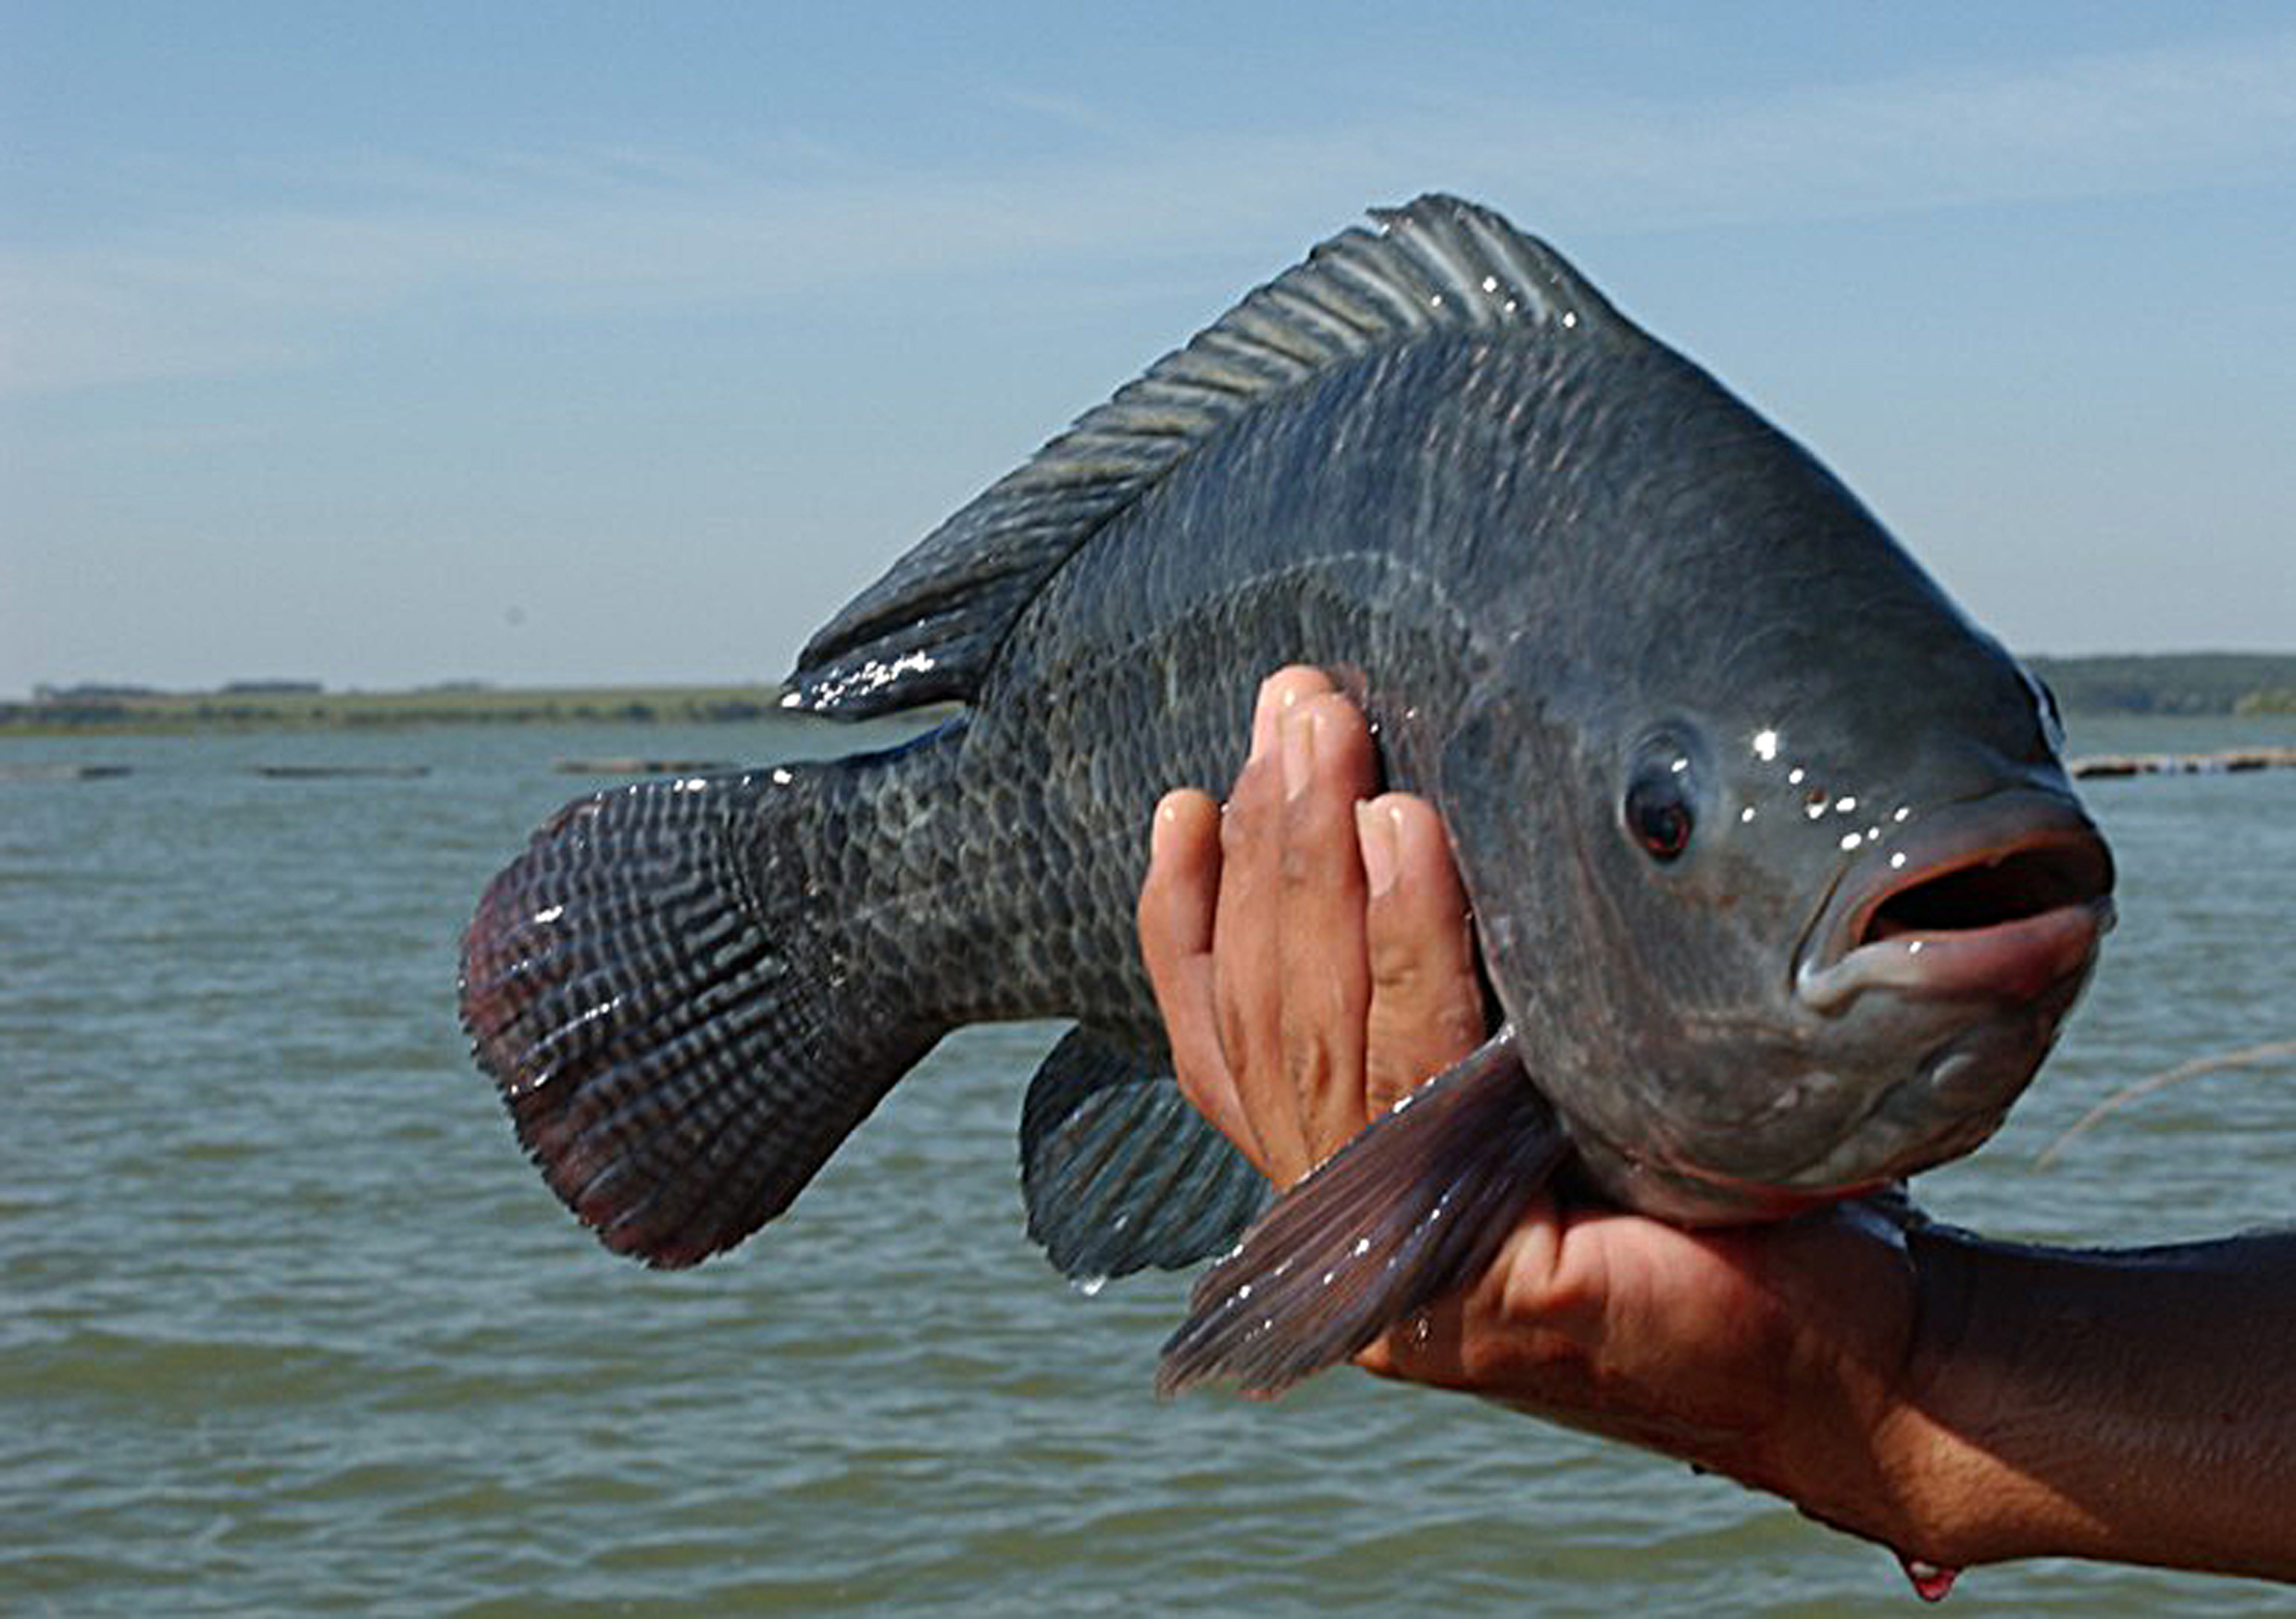
\includegraphics[scale=.5]{peixe.jpg}

\subsection{Formatação Avançada}

\begin{figure}[!h]
\centering
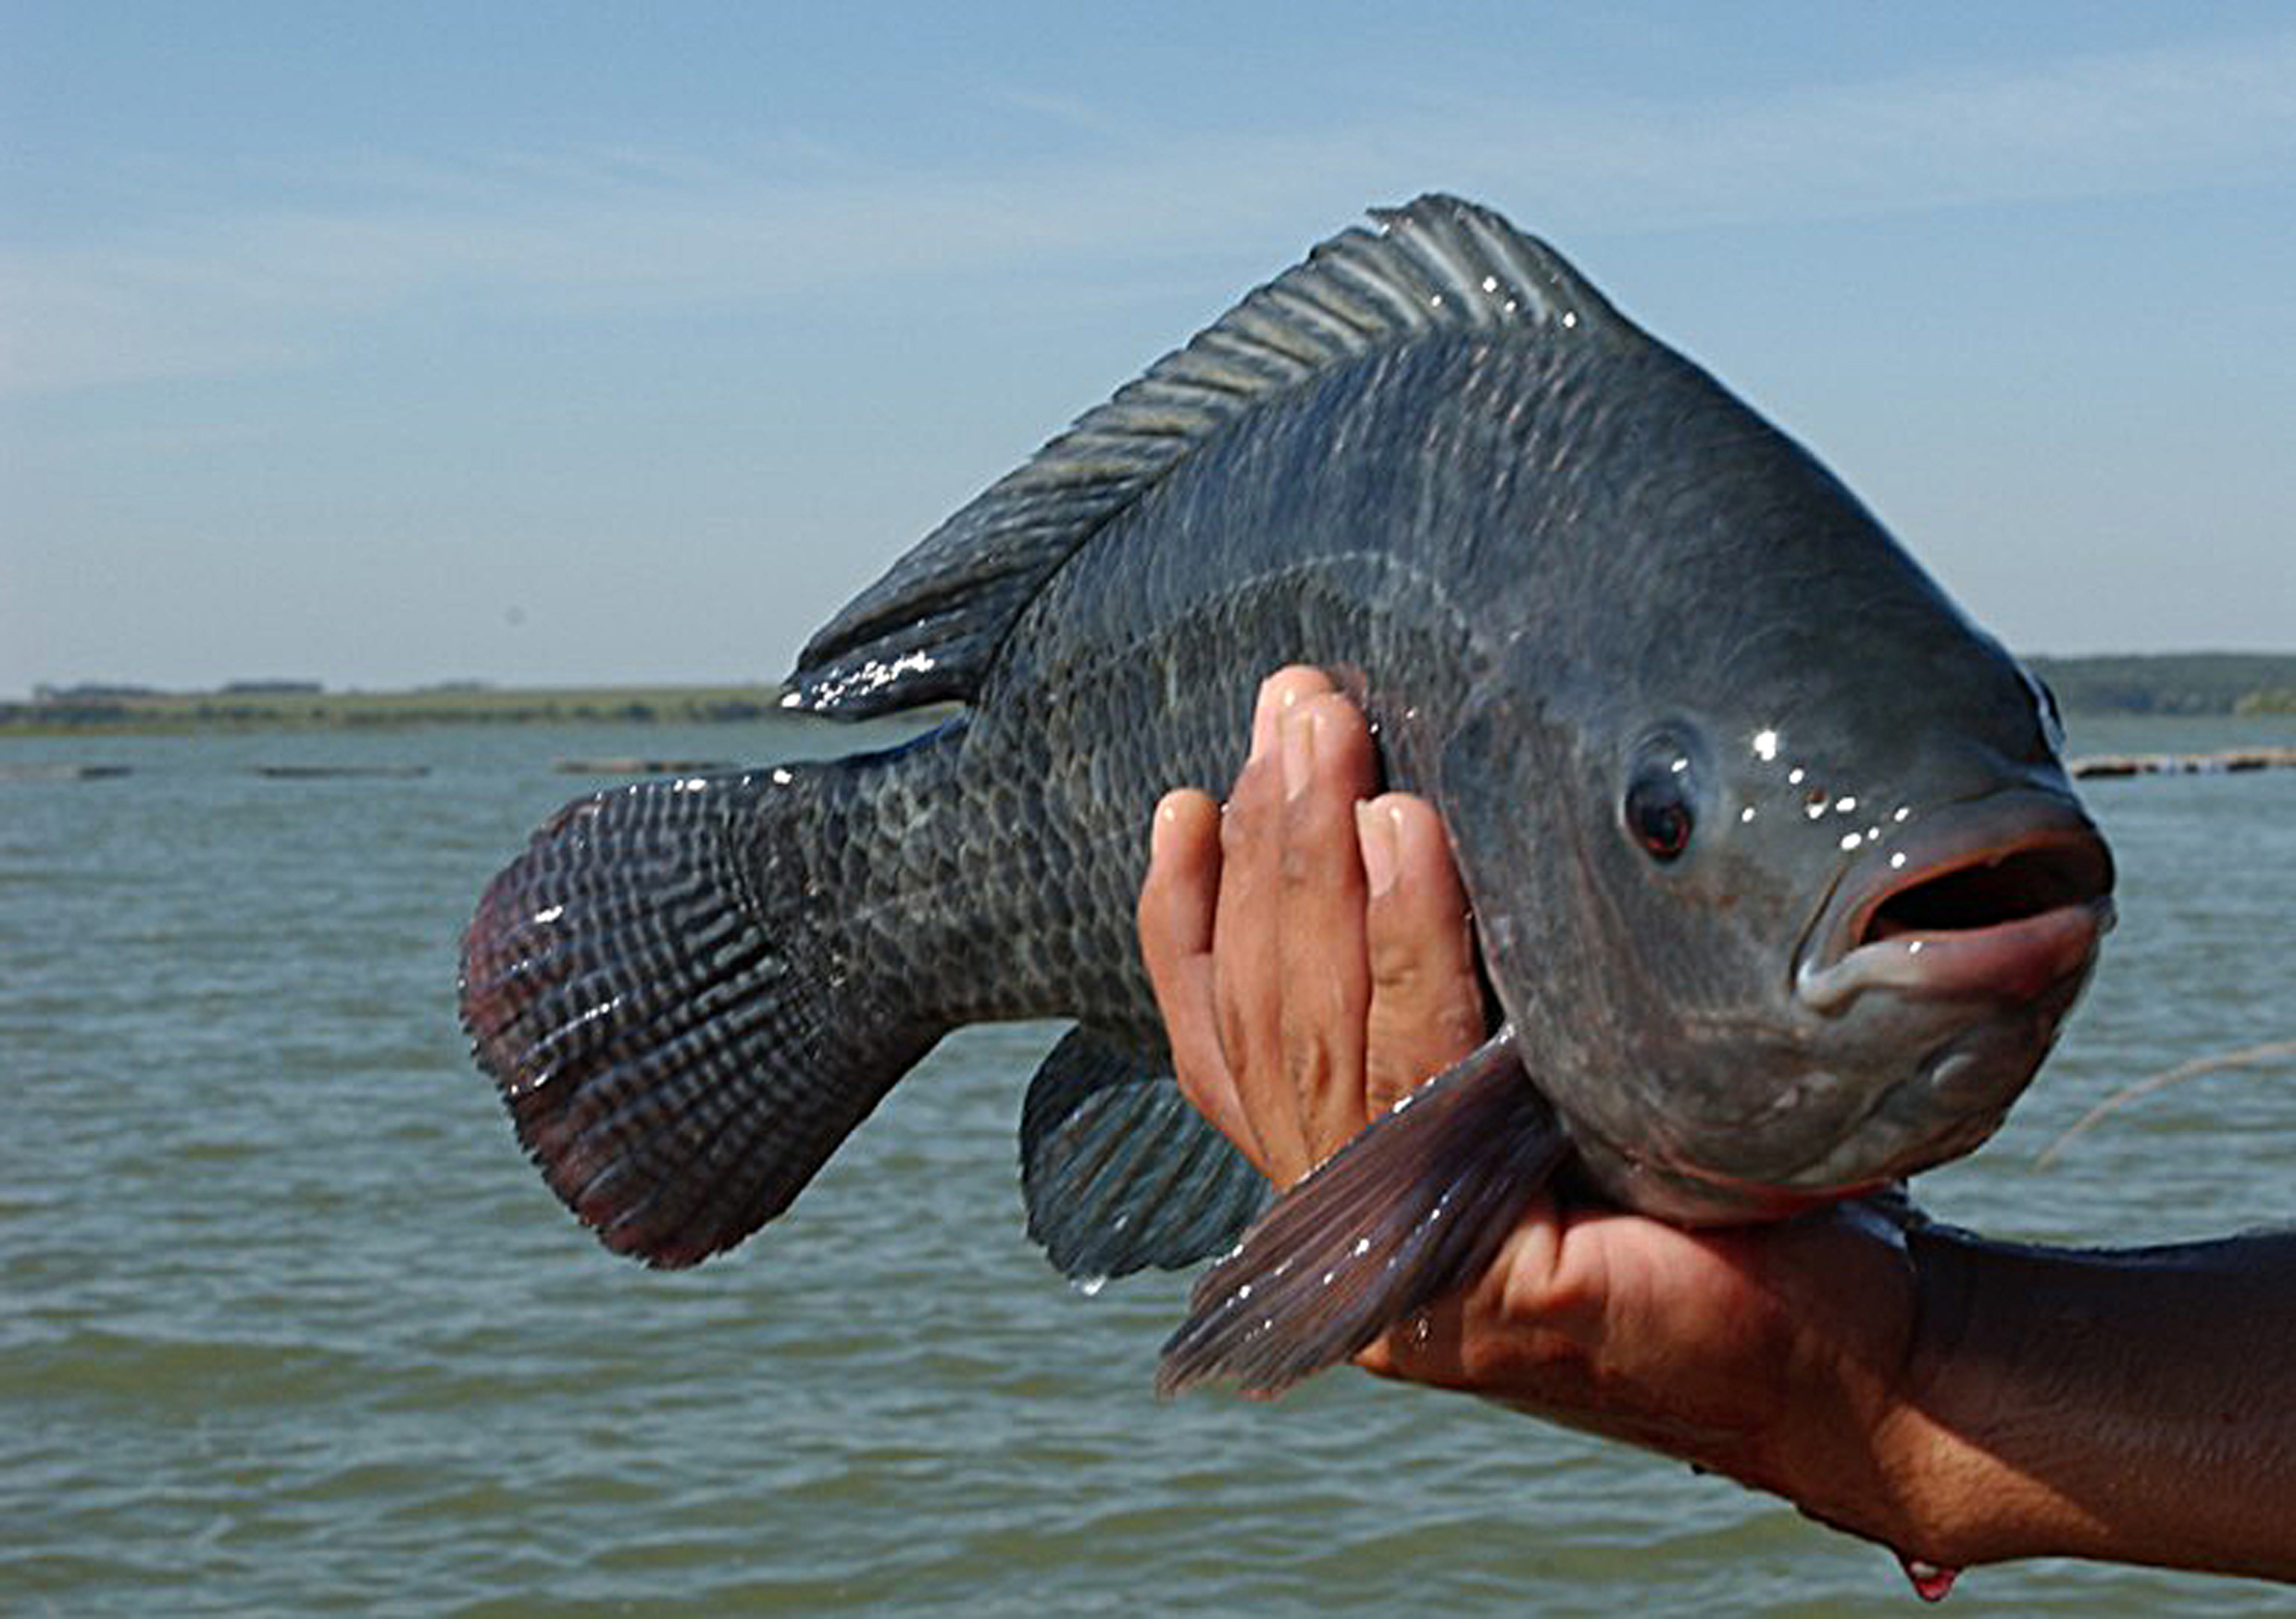
\includegraphics[width=.5\textwidth]{peixe.jpg}
\caption{Peixe Bonito}
\label{fig:pb}
\end{figure}

\section{Referenciando}
Na seção \ref{ssc:ldl} você viu como fazer uma lista dentro de outra, e a figura \ref{fig:pb} é um peixão bonito.

\begin{equation}
a^2 = b^2 + c^2
\label{eq:pit}
\end{equation}

A equação \eqref{eq:pit} é o Teorema de Pitágoras

\section{Matemática Alinhada}
\begin{align*}
f'(x) &= \lim_{h \to 0} \dfrac{f(x+h) - f(x)}{h}\\
d(\sin(x)) &= \lim_{h \to 0} \dfrac{\sin(x+h) - \sin(x)}{h}\\
 &= \lim_{h \to 0} \dfrac{\sin(x)\cdot \cos(h) + \sin(h)\cdot\cos(x) - \sin(x)}{h}\\
 &= \lim_{h \to 0} \dfrac{\sin(x)\cdot \cos(h)- \sin(x)}{h} + \dfrac{\sin(h)\cdot\cos(x)}{h}\\
 &= \lim_{h \to 0} \dfrac{\sin(x)(\cos(h)- 1)}{h} + \dfrac{\sin(h)\cdot\cos(x)}{h}\\
 &= \cos(x)
\end{align*}

\begin{align*}
a_1 &= 3 & a_n &= a_1 + (n-1)\cdot r\\
r &= 4 & a_{20} &= 3 + (20-1)\cdot 4\\
a_{20} &= ? & a_{20} &= 3 + 76 = 79\\
\end{align*}
\newpage
\section{Tabelas}
% Please add the following required packages to your document preamble:
% \usepackage{graphicx}
% \usepackage[table,xcdraw]{xcolor}
% If you use beamer only pass "xcolor=table" option, i.e. \documentclass[xcolor=table]{beamer}
\begin{table}[!h]
\centering
\resizebox{.9\textwidth}{!}{%
\begin{tabular}{|
>{\columncolor[HTML]{FD6864}}l |
>{\columncolor[HTML]{FFCCC9}}l |
>{\columncolor[HTML]{FFCCC9}}l |
>{\columncolor[HTML]{FFCCC9}}l |
>{\columncolor[HTML]{FFCCC9}}l |
>{\columncolor[HTML]{FFCCC9}}l |
>{\columncolor[HTML]{FFCCC9}}l |}
\hline
\cellcolor[HTML]{FE0000}{\color[HTML]{FFFFFF} \textbf{UF}} & \cellcolor[HTML]{FE0000}{\color[HTML]{FFFFFF} \textbf{Contaminados}} & \cellcolor[HTML]{FE0000}{\color[HTML]{FFFFFF} \textbf{Óbitos}} & \cellcolor[HTML]{FE0000}{\color[HTML]{FFFFFF} \textbf{\% Contaminada}} & \cellcolor[HTML]{FE0000}{\color[HTML]{FFFFFF} \textbf{Taxa de Mortalidade}} & \cellcolor[HTML]{FE0000}{\color[HTML]{FFFFFF} \textbf{Percentual Brasileiro}} & \cellcolor[HTML]{FE0000}{\color[HTML]{FFFFFF} \textbf{}} \\ \hline
{\color[HTML]{FFFFFF} AC}                                  & {\color[HTML]{000000} 404}                                           & {\color[HTML]{000000} 19}                                      & {\color[HTML]{000000} 0,0485}                                          & {\color[HTML]{000000} 4,700\%}                                              & {\color[HTML]{000000} 0,47\%}                                                 & {\color[HTML]{000000} 0,32\%}                            \\ \hline
{\color[HTML]{FFFFFF} AL}                                  & {\color[HTML]{000000} 1044}                                          & {\color[HTML]{000000} 47}                                      & {\color[HTML]{000000} 0,0312}                                          & {\color[HTML]{000000} 4,500\%}                                              & {\color[HTML]{000000} 1,22\%}                                                 & {\color[HTML]{000000} 0,80\%}                            \\ \hline
{\color[HTML]{FFFFFF} AM}                                  & {\color[HTML]{000000} 5254}                                          & {\color[HTML]{000000} 425}                                     & {\color[HTML]{000000} 0,1267}                                          & {\color[HTML]{000000} 8,089\%}                                              & {\color[HTML]{000000} 6,15\%}                                                 & {\color[HTML]{000000} 7,20\%}                            \\ \hline
{\color[HTML]{FFFFFF} AP}                                  & {\color[HTML]{000000} 1080}                                          & {\color[HTML]{000000} 34}                                      & {\color[HTML]{000000} 0,1277}                                          & {\color[HTML]{000000} 3,148\%}                                              & {\color[HTML]{000000} 1,26\%}                                                 & {\color[HTML]{000000} 0,58\%}                            \\ \hline
{\color[HTML]{FFFFFF} BA}                                  & {\color[HTML]{000000} 2851}                                          & {\color[HTML]{000000} 104}                                     & {\color[HTML]{000000} 0,0191}                                          & {\color[HTML]{000000} 3,647\%}                                              & {\color[HTML]{000000} 3,34\%}                                                 & {\color[HTML]{000000} 1,76\%}                            \\ \hline
{\color[HTML]{FFFFFF} CE}                                  & {\color[HTML]{000000} 7606}                                          & {\color[HTML]{000000} 482}                                     & {\color[HTML]{000000} 0,0832}                                          & {\color[HTML]{000000} 6,337\%}                                              & {\color[HTML]{000000} 8,91\%}                                                 & {\color[HTML]{000000} 8,17\%}                            \\ \hline
{\color[HTML]{FFFFFF} DF}                                  & {\color[HTML]{000000} 1356}                                          & {\color[HTML]{000000} 30}                                      & {\color[HTML]{000000} 0,0449}                                          & {\color[HTML]{000000} 2,212\%}                                              & {\color[HTML]{000000} 1,59\%}                                                 & {\color[HTML]{000000} 0,51\%}                            \\ \hline
{\color[HTML]{FFFFFF} ES}                                  & {\color[HTML]{000000} 2465}                                          & {\color[HTML]{000000} 83}                                      & {\color[HTML]{000000} 0,0613}                                          & {\color[HTML]{000000} 3,367\%}                                              & {\color[HTML]{000000} 2,89\%}                                                 & {\color[HTML]{000000} 1,41\%}                            \\ \hline
{\color[HTML]{FFFFFF} GO}                                  & {\color[HTML]{000000} 781}                                           & {\color[HTML]{000000} 29}                                      & {\color[HTML]{000000} 0,0111}                                          & {\color[HTML]{000000} 3,810\%}                                              & {\color[HTML]{000000} 0,91\%}                                                 & {\color[HTML]{000000} 0,49\%}                            \\ \hline
{\color[HTML]{FFFFFF} MA}                                  & {\color[HTML]{000000} 3190}                                          & {\color[HTML]{000000} 184}                                     & {\color[HTML]{000000} 0,045}                                           & {\color[HTML]{000000} 5,768\%}                                              & {\color[HTML]{000000} 3,74\%}                                                 & {\color[HTML]{000000} 3,12\%}                            \\ \hline
{\color[HTML]{FFFFFF} MG}                                  & {\color[HTML]{000000} 1827}                                          & {\color[HTML]{000000} 82}                                      & {\color[HTML]{000000} 0,0086}                                          & {\color[HTML]{000000} 4,488\%}                                              & {\color[HTML]{000000} 2,14\%}                                                 & {\color[HTML]{000000} 1,39\%}                            \\ \hline
{\color[HTML]{FFFFFF} MS}                                  & {\color[HTML]{000000} 255}                                           & {\color[HTML]{000000} 9}                                       & {\color[HTML]{000000} 0,0091}                                          & {\color[HTML]{000000} 3,529\%}                                              & {\color[HTML]{000000} 0,30\%}                                                 & {\color[HTML]{000000} 0,15\%}                            \\ \hline
{\color[HTML]{FFFFFF} MT}                                  & {\color[HTML]{000000} 297}                                           & {\color[HTML]{000000} 11}                                      & {\color[HTML]{000000} 0,0085}                                          & {\color[HTML]{000000} 3,700\%}                                              & {\color[HTML]{000000} 0,35\%}                                                 & {\color[HTML]{000000} 0,19\%}                            \\ \hline
{\color[HTML]{FFFFFF} PA}                                  & {\color[HTML]{000000} 2876}                                          & {\color[HTML]{000000} 208}                                     & {\color[HTML]{000000} 0,0334}                                          & {\color[HTML]{000000} 7,232\%}                                              & {\color[HTML]{000000} 3,37\%}                                                 & {\color[HTML]{000000} 3,52\%}                            \\ \hline
{\color[HTML]{FFFFFF} PB}                                  & {\color[HTML]{000000} 814}                                           & {\color[HTML]{000000} 62}                                      & {\color[HTML]{000000} 0,0202}                                          & {\color[HTML]{000000} 7,610\%}                                              & {\color[HTML]{000000} 0,95\%}                                                 & {\color[HTML]{000000} 1,05\%}                            \\ \hline
{\color[HTML]{FFFFFF} PE}                                  & {\color[HTML]{000000} 6876}                                          & {\color[HTML]{000000} 565}                                     & {\color[HTML]{000000} 0,0719}                                          & {\color[HTML]{000000} 8,217\%}                                              & {\color[HTML]{000000} 8,05\%}                                                 & {\color[HTML]{000000} 9,57\%}                            \\ \hline
{\color[HTML]{FFFFFF} PI}                                  & {\color[HTML]{000000} 513}                                           & {\color[HTML]{000000} 24}                                      & {\color[HTML]{000000} 0,0156}                                          & {\color[HTML]{000000} 4,670\%}                                              & {\color[HTML]{000000} 0,60\%}                                                 & {\color[HTML]{000000} 0,41\%}                            \\ \hline
{\color[HTML]{FFFFFF} PR}                                  & {\color[HTML]{000000} 1407}                                          & {\color[HTML]{000000} 83}                                      & {\color[HTML]{000000} 0,0123}                                          & {\color[HTML]{000000} 5,899\%}                                              & {\color[HTML]{000000} 1,65\%}                                                 & {\color[HTML]{000000} 1,41\%}                            \\ \hline
{\color[HTML]{FFFFFF} RJ}                                  & {\color[HTML]{000000} 9453}                                          & {\color[HTML]{000000} 854}                                     & {\color[HTML]{000000} 0,0547}                                          & {\color[HTML]{000000} 9,030\%}                                              & {\color[HTML]{000000} 11,07\%}                                                & {\color[HTML]{000000} 14,47\%}                           \\ \hline
{\color[HTML]{FFFFFF} RN}                                  & {\color[HTML]{000000} 1177}                                          & {\color[HTML]{000000} 56}                                      & {\color[HTML]{000000} 0,0335}                                          & {\color[HTML]{000000} 4,757\%}                                              & {\color[HTML]{000000} 1,38\%}                                                 & {\color[HTML]{000000} 0,95\%}                            \\ \hline
{\color[HTML]{FFFFFF} RO}                                  & {\color[HTML]{000000} 502}                                           & {\color[HTML]{000000} 16}                                      & {\color[HTML]{000000} 0,282}                                           & {\color[HTML]{000000} 3,187\%}                                              & {\color[HTML]{000000} 0,59\%}                                                 & {\color[HTML]{000000} 0,27\%}                            \\ \hline
{\color[HTML]{FFFFFF} RR}                                  & {\color[HTML]{000000} 519}                                           & {\color[HTML]{000000} 7}                                       & {\color[HTML]{000000} 0,0856}                                          & {\color[HTML]{000000} 1,348\%}                                              & {\color[HTML]{000000} 0,61\%}                                                 & {\color[HTML]{000000} 0,12\%}                            \\ \hline
{\color[HTML]{FFFFFF} RS}                                  & {\color[HTML]{000000} 1466}                                          & {\color[HTML]{000000} 51}                                      & {\color[HTML]{000000} 0,0128}                                          & {\color[HTML]{000000} 3,478\%}                                              & {\color[HTML]{000000} 1,72\%}                                                 & {\color[HTML]{000000} 0,86\%}                            \\ \hline
{\color[HTML]{FFFFFF} SC}                                  & {\color[HTML]{000000} 2085}                                          & {\color[HTML]{000000} 46}                                      & {\color[HTML]{000000} 0,0291}                                          & {\color[HTML]{000000} 2,206\%}                                              & {\color[HTML]{000000} 2,44\%}                                                 & {\color[HTML]{000000} 0,78\%}                            \\ \hline
{\color[HTML]{FFFFFF} SE}                                  & {\color[HTML]{000000} 447}                                           & {\color[HTML]{000000} 12}                                      & {\color[HTML]{000000} 0,194}                                           & {\color[HTML]{000000} 2,684\%}                                              & {\color[HTML]{000000} 0,52\%}                                                 & {\color[HTML]{000000} 0,20\%}                            \\ \hline
{\color[HTML]{FFFFFF} SP}                                  & {\color[HTML]{000000} 28698}                                         & {\color[HTML]{000000} 2375}                                    & {\color[HTML]{000000} 0,0624}                                          & {\color[HTML]{000000} 8,275\%}                                              & {\color[HTML]{000000} 33,61\%}                                                & {\color[HTML]{000000} 40,25\%}                           \\ \hline
{\color[HTML]{FFFFFF} TO}                                  & {\color[HTML]{000000} 137}                                           & {\color[HTML]{000000} 3}                                       & {\color[HTML]{000000} 0,0087}                                          & {\color[HTML]{000000} 2,189\%}                                              & {\color[HTML]{000000} 0,16\%}                                                 & {\color[HTML]{000000} 0,05\%}                            \\ \hline
{\color[HTML]{FFFFFF} BR}                                  & {\color[HTML]{000000} 85380}                                         & {\color[HTML]{000000} 5901}                                    & {\color[HTML]{000000} }                                                & {\color[HTML]{000000} }                                                     & {\color[HTML]{000000} 100,00\%}                                               & {\color[HTML]{000000} 100,00\%}                          \\ \hline
\end{tabular}%
}
\caption{Tabela COVID}
\label{tab:tabela}

\end{table}
\begin{table}[!h]
\centering
\resizebox{.6\textwidth}{!}{%
\begin{tabular}{@{}cccc@{}}
\toprule
Nome                          & Curso                          & Idade                   & SO                            \\ \midrule
\multicolumn{1}{|c|}{Eduardo} & \multicolumn{1}{c|}{Téc. Mec.} & \multicolumn{1}{c|}{17} & \multicolumn{1}{c|}{MX Linux} \\ \midrule
                              &                                &                         &                               \\ \bottomrule
\end{tabular}%
}
\caption{Relação de SO e Curso por Aluno}
\label{tab:my-table}
\end{table}


\end{document}